\subsection{Прецессия}

Ось вращения Земли совершает прецессионное движение --- описывает вокруг оси эклиптики  конус радиусом основания 23.5$^\circ$ с периодом около 26 000 лет. Из-за этого меняется положение полюс мира. Например, сейчас полюс мира практически совпадает с Полярной звездой ($\alpha$ Малой Медведицы), а 15 000 лет назад роль Полярной звезды играла Вега ($\alpha$ Лиры). Если считать, что величина прецессии постоянна, то полюсы мира описывают вокруг полюсов эклиптики малые круги с радиусом 23.5$^\circ$. В действительности же величина прецессии меняется, поэтому путь полюсов мира представляет собой не окружность, а спираль.

Поворот оси Земли имеет различные последствия. Во-первых, меняется продолжительность тропического года, он становится примерно на 20 минут короче звёздного. Во-вторых, из-за прецессии меняется вид звёздного неба, хотя происходит это очень медленно (Рис.12).
\begin{center}
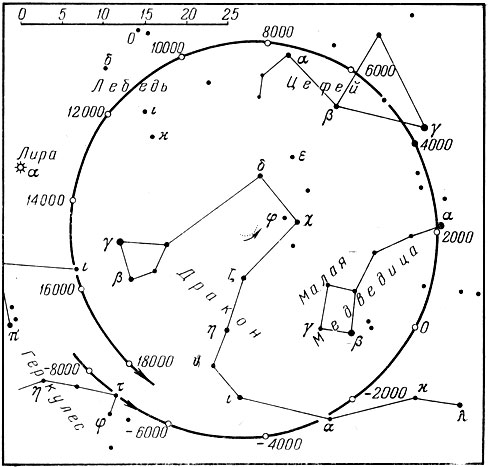
\includegraphics[scale=0.46]{Precession}
\begin{figure}[h!]
\caption{Прецессионное движение северного полюса мира}
\end{figure}
\end{center}